\begin{figure}[htbp]
\section*{ LZTR1}
\centering
\begin{subfigure}[b]{0.95\textwidth}
\centering
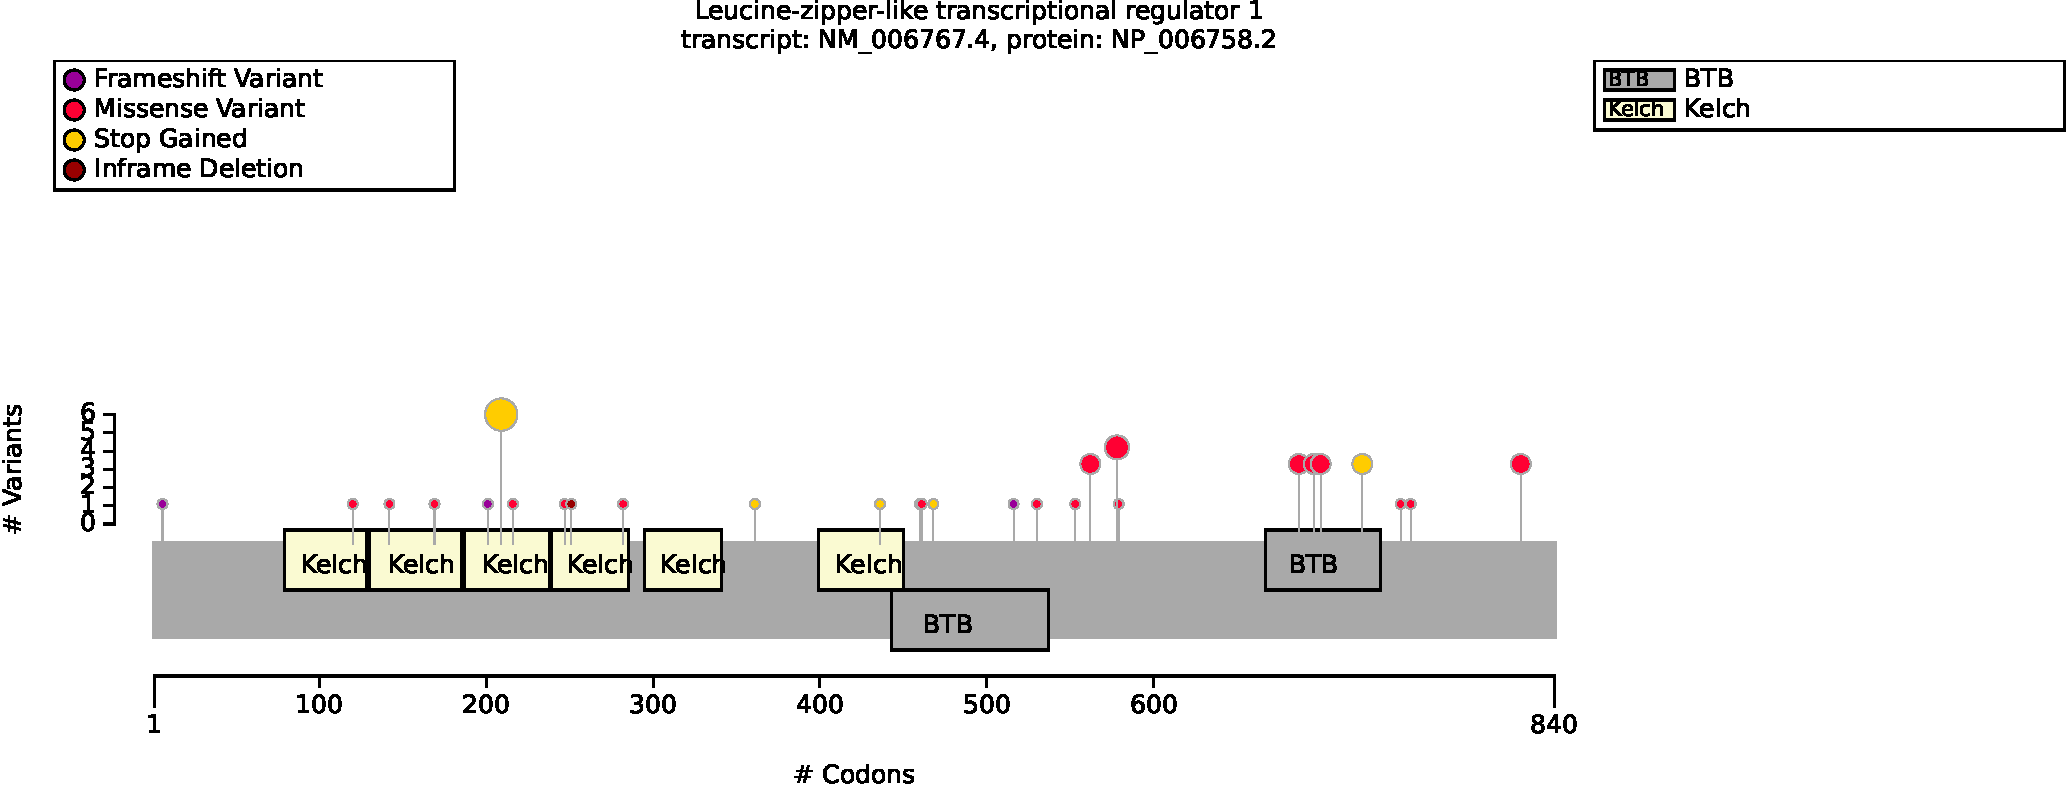
\includegraphics[width=\textwidth]{ img/LZTR1_protein_diagram.pdf} 
\captionsetup{justification=raggedright,singlelinecheck=false}
\caption{Distribution of variants in LZTR1}
\end{subfigure}

\vspace{2em}

\begin{subfigure}[b]{0.95\textwidth}
\centering
\resizebox{\textwidth}{!}{
\begin{tabular}{llllrr}
\toprule
Genotype (A) & Genotype (B) & total tests performed & significant results\\
\midrule
N Term/N Term OR N Term/Other & Other/Other & 49 & 0\\
Missense/Missense OR Missense/Other & Other/Other & 49 & 0\\
FEMALE & MALE & 54 & 0\\
\bottomrule
\end{tabular}
}
\captionsetup{justification=raggedright,singlelinecheck=false}
\caption{ Fisher Exact Test performed to compare HPO annotation frequency with respect to genotypes. }
\end{subfigure}

\vspace{2em}

\caption{ The cohort comprised 38 individuals (18 females, 20 males). 3 of these individuals were reported to be deceased. A total of 96 HPO terms were used to annotate the cohort. Disease diagnosis: Noonan syndrome 2 (OMIM:605275). No significant association identified. A total of 38 unique variant alleles were found in \textit{LZTR1} (transcript: \texttt{NM\_006767.4}, protein id: \texttt{NP\_006758.2}).}
\end{figure}
